
\section{Linear Programming}

Linear programming is an optimisation problem, where we want to find the `best'
solution to a set of equations. We're going to solve it using the
\textit{simplex} method, but before we do, I think it's a good idea to recap
some high-school mathematics first. Feel free to skip the next subsection if
you're feeling confident with it.

\subsection{Background mathematics}

An inequality relation is just like a normal equation, except the equals sign is
replaced by either $<$, $>$, $\leq$ or $\geq$. When you solve an inequality, you
generally want to get all of the similar terms on one side (e.g. move all the
variable terms over to one side, and all of the constants to another side). This
\textit{mostly} works like a normal equation; you can add and subtract from both
sides just like normal, however, if you want to divide or multiply \textbf{by a
negative quantity}, then you need to \textbf{reverse the equality}, for example:

\[
  \begin{split}
    -2x &> -2\\
    2x &< 2\\
    x &< 1
  \end{split}
\]

This equality is satisfied whenever $x$ is less than $1$. If we have two terms
in the equality (something similar to $ax + by \geq c$), it becomes slightly
harder to solve. To solve this we can:

\begin{itemize}
  \item Plot a graph of the line $ax + by = c$.
  \item Pick a test point $(x, y)$ not on the line, and plot it on the graph.
  \item If the point $(x, y)$ satisfies the inequality, then shade the opposite 
    side of the line to which the point is on, otherwise, shade the same side.
\end{itemize}

For example, given $3x + 4y \leq 6$, and choosing the point $(-2,1)$ we end up
with what's in Figure~\ref{fig:graph-1}.

\begin{figure}[h]
  \centering
  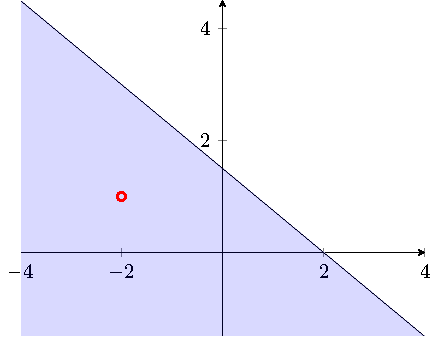
\includegraphics{diagrams/graph1}
  \caption{A graph of $3x + 4y \leq 6$, with all the valid values shaded blue.}
  \label{fig:graph-1}
\end{figure}

If we have multiple inequalities, we want to \textit{find the region where all
of them are satisfied}. This involves plotting each line, and shading the
regions where they're not satisfied, which means the blank bit is the bit we
want.

If we have the equations $3x + 4y \leq 6$, $2y - x \leq 2$ and $x \geq 0$, we
will get something like in Figure~\ref{fig:graph-2}.

\begin{figure}[H]
\captionsetup{width=.4\linewidth}
\centering
\begin{minipage}{.45\textwidth}
  \centering
  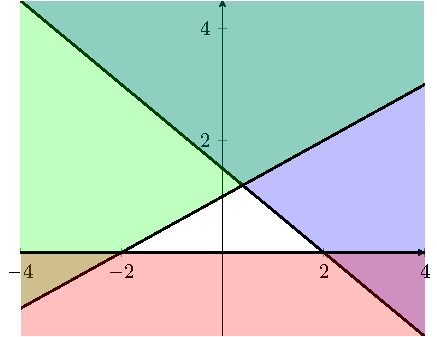
\includegraphics[width=\textwidth]{diagrams/graph2}
  \captionof{figure}{A graph plotting $3x + 4y \leq 6$, $2y - x \leq 2$ and
  $x \geq 0$, where the points not satisfying the inequalities are shaded in 
  blue, green and red respectively. The clear region satisfies all points.}
  \label{fig:graph-2}
\end{minipage}%
\begin{minipage}{.45\textwidth}
  \centering
  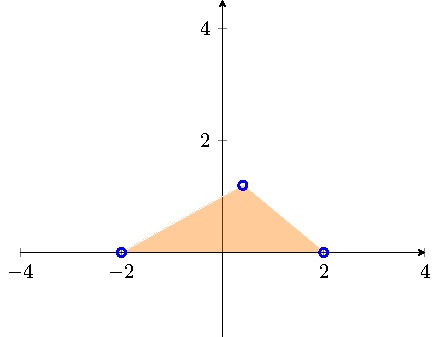
\includegraphics[width=\textwidth]{diagrams/graph3}
  \captionof{figure}{The valid region in the three inequalities from
  Figure~\ref{fig:graph-2}. The corner points are $(2,0),(-2,0)$ and
  $(\frac{2}{5},\frac{6}{5})$.}
  \label{fig:graph-3}
\end{minipage}
\end{figure}


The corner points are especially important to us, since that's often where the
useful numbers are (we'll see more of this later). In order to find the corner
points, we solve the two lines that form them. Solving the following equations
gives the points in Figure~\ref{fig:graph-3}.

\begin{mymulticols}
  \begin{itemize}
    \item $x = 0,~3x + 4y = 6$
    \item $x = 0,~2y - x = 2$
    \item $2y - x = 2,~3x + 4y = 6$
  \end{itemize}
\end{mymulticols}

So, now we know how to solve these types of problems, lets look at how to
decompose a problem statement into a set of equations.

\begin{quote}

  You can buy wood in 11 meter lengths, or 6 meter lengths. A 11 meter piece of
  wood can be cut into two lengths of 5 meters, and one length of 1 meter. A 6
  meter piece of wood is cut into one length of 5 meter, and one length of 1
  meter.

  If we have room for twenty 1 meter pieces and thirty 5 meter pieces, how many
  11, and how many 6 meter lengths should we buy? We cannot go over that amount
  of pieces, but we can settle for less than that amount.

\end{quote}

To answer this, we can make a table to describe it:

\begin{center}
  \begin{tabular} {|p{3cm}|p{2cm}|p{2cm}|}
    \hline
    \multirow{2}{*}{Bought Length} & \multicolumn{2}{c|}{Required length}\\
    \cline{2-3}
    & 5 meter & 1 meter\\ \hline
    11 meter (x)\newline 6 meter (y) & 2 per board\newline 1 per board & 1 per
    board\newline 1 per board\\ \hline
    Amount needed & 30 & 20\\ \hline
  \end{tabular}
\end{center}

This decomposes into the following equations:

\begin{itemize}
  \item $2x + y \leq 30$
  \item $x + y \leq 20$
  \item $x \geq 0$, $y \geq 0$
\end{itemize}

\marginpar{Notice how our shapes always have a convex hull...}

Plotting this on a graph gives us what's in Figure~\ref{fig:graph-4}, where we
can see a feasible region between $(0, 20), (10, 10), (15, 0)$ and  $(0,0)$. The
three corner points are all of the non-zero points (zero eleven meter and zero
six meter pieces is an invalid solution), and anywhere on the outer edge of the
region is a solution.

\begin{figure}[h]
  \centering
  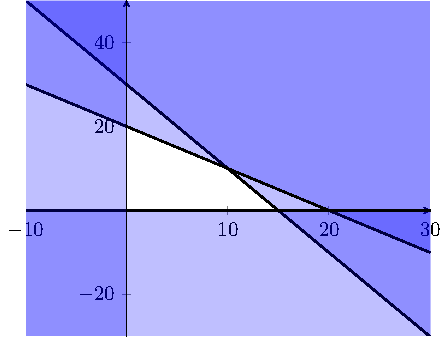
\includegraphics{diagrams/graph4}
  \caption{A graph of $2x + y = 30$, $x + y = 20$, $x > 0$, $y > 0$.}
  \label{fig:graph-4}
\end{figure}

\subsection{The maximum problem}

Sometimes, we want to maximise some particular variable. For example, companies
want to maximise their profit. If this is the case, then we can come up with a
function for the profit, something like:

\[
  P = 7x + 3y
\]

Where $x$ is the number of $5$ meter boards, and $y$ is the number of $1$ meter
boards. We can factor this equation into our solution, to find the most
profitable wood to buy.

If you think about it, the further from the origin we get, the more profit (in
this instance) we get. At $(0,0)$ we have no profit, since we have done nothing,
but at $(5,0)$ we have $35$ profit since we have bought five, $5$ meter length
boards. Since our lines always intersect to produce a region with a convex
shape, the points furthest from the origin are the corner points. To figure out
how much profit we can make, we just need to find the maximum of these points:

\begin{center}
  \begin{tabular}{c | c | c | c}
    \textbf{Corner point} & \textbf{5 meter boards} & \textbf{1 meter boards}
      & \textbf{Profit}\\  \hline
    $(0,20)$  & 20 & 20 & 200\\ \hline
    $(10,10)$ & 30 & 20 & 270\\ \hline
    $(15,0)$  & 30 & 15 & 255\\
  \end{tabular}
\end{center}

Therefore the most profitable choice is to buy $10$ 11 meter length boards and
$10$ 6 meter length boards.

\subsubsection{Matrix form}

We can put problems into another form; matrix form, and solve them that way.
Here is the example from the
\href{https://en.wikipedia.org/wiki/Linear_programming}{Linear programming
wikipedia article}.

\begin{figure}[H]
  \centering
  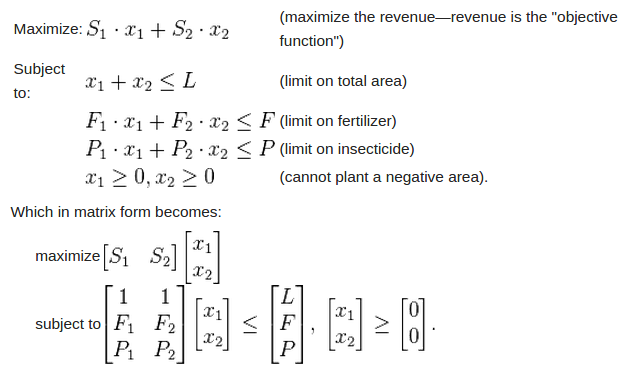
\includegraphics[width=0.7\textwidth]{images/matrix}
  \caption{Putting a LP problem into matrix form.}
  \label{matrixform}
\end{figure}

\subsection{The Simplex Method}

If we have more than two variables, then all of a sudden, working out the
optimum on a graph becomes rather hard. Drawing 3d graphs is hard, and
visualising n-dimensional graphs quickly becomes infeasible.

The simplex method automates finding the optimum value of any number of
variables. This is how it works:

\begin{itemize}
  \item Draw the feasible region in $n$ dimensional space
  \item Select a corner of the feasible region
  \item Choose an edge that is connected to this point that will increase the
  objective function.
  \item Go to the next corner on that edge
  \item Keep doing steps 3 and 4 until you find an optimal solution.
\end{itemize}

That's pretty far removed from how we see the simplex algorithm working, since
we find the optimum by using a tableaux. I've broken down the algorithm into
multiple steps with a running example here:

\begin{itemize}
  \item[\textbf{Step 0}] The zero'th step, is to examine the input data we're 
  given. This will consist of a function $f$ to be maximised and a set of 
  inequalities that constrain the values we can give to $f$.

  \[\begin{split}
    f &= 10x + 12y +12z\\
    3 &\geq 5x + 2y + z\\
    2&\geq x + 2y + 4z\\
  \end{split}\]

  N.b. if the inequalities aren't of the form $CONST \geq EXPR$, then rearrange 
  them so that they are.

  \item[\textbf{Step 1}] Now we turn each inequality we were given into an 
  equation (replace the inequality sign with an equals basically), and introduce 
  a new variable for each (called a \textit{slack variable}). Also, rearrange
  $f$ so its equal to zero:

  \begin{alignat*}{12}
    3 &=~ &5x~  &+~&2y~ &+~&z ~&+~&m_1&~ &~  &~ &~  &~&~\\
    2 &=~ &~x   &+~&2y~ &+~& z~&~~&~  &+~&m_2&~ &~  &~&~\\
    0 &=~ &-10x~&-~&12y~&-~&12z&~ &~  &~ &~  &~ &~  &+&f
  \end{alignat*}
  \item[\textbf{Step 2}] Now our problem is in the correct form, we can whack it 
  into a tableaux:

  \begin{center}
    \begin{tabular}{>{$}c<{$}|>{$}c<{$}|>{$}c<{$}|>{$}c<{$}|>{$}c<{$}|
      >{$}c<{$}|>{$}c<{$}|>{$}c<{$}|>{$}c<{$}}
          & x & y & z & m_1 & m_2 & m_3 & f & \text{constants}\\ \hline
      m_1 & 5 & 2 & 1 & 1   & 0   & 0   & 0   & 3\\ \hline
      m_2 & 1 & 2 & 4 & 0   & 1   & 0   & 0   & 2\\ \hline
      f   &-10&-12&-12& 0   & 0   & 0   & 1   & 0\\
    \end{tabular}
  \end{center}

  It should be quite obvious how we go from the equations in step 1 to the
  tableaux in here. The only stuff you need to \textit{remember} about
  formatting the tableaux, is that the slack variables go along the left side,
  $f$ is the bottom row, and to put the constants in the last column.

  The values in the bottom row are called \textbf{indicators}.

  \item[\textbf{Step 3}] We need to find the \textbf{pivot cell} in the table. 
  The pivot column is easy to find, its the one with the most negative 
  indicator (in our case, the second or third column, since the indicators 
  there are $-12$, we're picking column two for no particular reason). 
  Finding the row is a bit harder, you need to divide the constant column by 
  the pivot column and pick the one with the lowest value:

  \marginpar{\textbf{Only choose positive ratios}, and remember that
  $?/0 = \infty$. Otherwise it goes belly up and it takes you over a day to 
  figure out why (this may or may not have  happened to me...).}

  \definecolor{highlight}{gray}{0.7}
  \definecolor{dhighlight}{gray}{0.5}

  \begin{center}
    \begin{tabular}{>{$}c<{$}|>{$}c<{$}|
      >{$}>{\columncolor{highlight}}c<{$}|>{$}c<{$}|>{$}c<{$}|
      >{$}c<{$}|>{$}c<{$}|>{$}c<{$}|>{$}c<{$}|c}
          & x & y & z & m_1 & m_2 & m_3 & f & \text{constants}
            & \text{ratio}\\ \hline
      m_1 & 5 & 2                       & 1 &1& 0& 0&0&3 & 3/2 \\ \hline
      \rowcolor{highlight}
      m_2 & 1 &\cellcolor{dhighlight} 2 & 4 &0& 1& 0&0&2 & 2/2\\ \hline
      f   &-10&-12                      &-12&0& 0& 0&1&0 & N/A \\
    \end{tabular}
  \end{center}

  \item[\textbf{Step 4}] Now we do the pivot about the pivot cell:

    \begin{itemize}
      \item[\textbf{Step 4a}] Divide each cell in the pivot's row by the pivot
      (which makes the pivot equal to $1$!).

      \begin{center}
        \renewcommand{\arraystretch}{1.2}
        \begin{tabular}{>{$}c<{$}|>{$}c<{$}|
          >{$}c<{$}|>{$}c<{$}|>{$}c<{$}|
          >{$}c<{$}|>{$}c<{$}|>{$}c<{$}|>{$}c<{$}}
              & x & y & z & m_1 & m_2 & m_3 & f & \text{constants}\\ \hline
          m_1 & 5 & 2 & 1 &1& 0& 0&0&3\\ \hline
          \rowcolor{highlight}
          m_2&\frac{1}{2}&\cellcolor{dhighlight}1&2&0&\frac{1}{2}&0&0&1\\ \hline
          f   &-10&-12&-12&0& 0& 0&1&0\\
        \end{tabular}
      \end{center}

      \item[\textbf{Step 4b}] Subtract the pivot row from each other row
      so that the whole pivot column becomes $0$. For example here, we need to
      make $R1 = R1 - 2(R2), R3 = R3 + 12(R2)$ to make the cell below 
      the pivot $0$.

      \begin{center}
        \renewcommand{\arraystretch}{1.2}
        \begin{tabular}{>{$}c<{$}|>{$}c<{$}|
          >{$}c<{$}|>{$}c<{$}|>{$}c<{$}|
          >{$}c<{$}|>{$}c<{$}|>{$}c<{$}|>{$}c<{$}}
              & x & y & z & m_1 & m_2 & m_3 & f & \text{constants}\\ \hline
          m_1 & 4 & 0 &-3 &1&-1& 0&0&1\\ \hline
          m_2 & \frac{1}{2} & 1& 2 &0&\frac{1}{2}&0&0&1\\ \hline
          f   &-4 & 0 & 12&0& 6& 0&1&12\\
        \end{tabular}
      \end{center}

      \item[\textbf{Step 4c}] Replace the letter on the pivot row with the 
      letter on the pivot column:

      \begin{center}
        \renewcommand{\arraystretch}{1.2}
        \begin{tabular}{>{$}c<{$}|>{$}c<{$}|
          >{$}c<{$}|>{$}c<{$}|>{$}c<{$}|
          >{$}c<{$}|>{$}c<{$}|>{$}c<{$}|>{$}c<{$}}
              & x & y & z & m_1 & m_2 & m_3 & f & \text{constants}\\ \hline
          m_1 & 4 & 0 &-3 &1&-1& 0&0&1\\ \hline
          y & \frac{1}{2} & 1& 2 &0&\frac{1}{2}&0&0&1\\ \hline
          f   &-4 & 0 & 12&0& 6& 0&1&12\\
        \end{tabular}
      \end{center}
    \end{itemize}

    \item[\textbf{Step 5}] Now we have found another solution, to see what it 
    is, read off the letters on the far left and correspond them to the 
    constants on the far right:

    \[
      x = 0, y = 1, z = 0, m_1 = 1, m_2 = 0, f = 12
    \]

    If we sub that in, then we can see that if satisfies the formulae from step
    1:

    \begin{alignat*}{12}
      3 &=~ & 0~  &+~&2~ &+~&0 ~&+~&  1&~ &~  &~ &~  &~&~\\
      2 &=~ &~0   &+~&2~ &+~&0 ~&~~&~  &+~&  0&~ &~  &~&~\\
      0 &=~ &-0  ~&-~&12~&-~&0  &~ &~  &~ &~  &~ &~  &+&12
    \end{alignat*}

  \item[\textbf{Step 6}] If there are no negative indicators in the table
  (bottom row of the tableaux), then we've finished, and our solution is the 
  optimal one. If there are, then we need to go back to step 3 and repeat until 
  there aren't any negative indicators. Since we have a negative indicator in 
  the first column, then we should loop back and do another iteration.

\end{itemize}

If we run steps 3-6 again (which we should do because there is a
negative indicator), we get the optimum, which is:

\begin{center}
  \renewcommand{\arraystretch}{1.2}
  \begin{tabular}{>{$}c<{$}|>{$}c<{$}|
    >{$}c<{$}|>{$}c<{$}|>{$}c<{$}|
    >{$}c<{$}|>{$}c<{$}|>{$}c<{$}|>{$}c<{$}}
        & x & y & z & m_1 & m_2 & m_3 & f & \text{constants}\\ \hline
    x & 1 & 0 &\frac{-3}{4}&\frac{1}{4} &\frac{-1}{4}&0&0&\frac{1}{4}\\ \hline
    y & 0 & 1 &\frac{19}{8}&\frac{-1}{8}&\frac{5}{8} &0&0&\frac{7}{8}\\ \hline
    f & 0 & 0 & 9          & 1          & 5          &0&0&13\\
  \end{tabular}
\end{center}

So:

\[
  f = 13,~x = 0.25,~y = 0.825,~z = 0
\]

You can use this tool to check solutions to simplex problems:
\url{http://www.zweigmedia.com/RealWorld/simplex.html}.

\subsubsection{Duality}

Simplex is great if we're trying to maximise a function, but what if we want to
minimise it? Duality does this. Basically, you give it a function and
inequalities, it mutates them so they'll fit into simplex, and then you run
simplex as normal. So, to apply the duality theorem, you need:

\begin{itemize}
  \item A function you want to minimize; $f = ax + by + \dots$
  \item A set of inequalities of the form `$EXPR \geq CONST$'
\end{itemize}

Since simplex tries to maximise $f$, which is the opposite of what we want to
do, and our inequalities are the wrong way around, we need to the duality bit
now:

First, like the first part of simplex, we put the coefficients in a table.
However, this table has a special name; the \textit{coefficient matrix}. It's
called a matrix, not a table because we're going to do a transposition on it
(and mathematicians transpose matrices, not tables!). 

The input:

\[
  \begin{split}
    g = 3r + 4s + t\\
    r + 2s + t \geq 4\\
    r + 2s - t \geq -2\\
    r + s \geq -1\\
    r \geq 0,~s \geq 0,~t \geq 0
  \end{split}
\]

Would result in a matrix like this:

\begin{center}
  \begin{tabular}{>{$}r<{$}|>{$}c<{$} >{$}c<{$} >{$}c<{$} >{$}l<{$}}
        & r & s & t & \text{constants}\\ \hline
        & 1 & 2 & 1 &4\\ 
        & 1 & 2 &-1 &-2\\ 
        & 1 & 1 & 0 &-1\\ 
      g & 3 & 4 & 1 &  \\ 
  \end{tabular}
\end{center}

So, we put the inequalities in first, then put the minimising function in the
last column. Now what we do, is to flip the matrix along its top-left to bottom-
right diagonal:

\begin{center}
  \begin{tabular}{>{$}r<{$}|>{$}c<{$} >{$}c<{$} >{$}c<{$} >{$}l<{$}}
        & x & y & z & \text{constants}\\ \hline
        & 1 & 1 & 1 & 3\\ 
        & 2 & 2 & 1 & 4\\ 
        & 1 &-1 & 0 & 1\\ 
      f & 4 &-2 &-1 &  \\ 
  \end{tabular}
\end{center}

After we've done that, we get the following equation and inequalities:

\[
  \begin{split}
    f = 4x - 2y - z\\
    x + y + z \leq 3\\
    2x + 2y + z \leq 4\\
    x - y \leq 1\\
    x \geq 0, y \geq 0,~z \geq 0
  \end{split}
\]

If you do simplex on them (you should try it for practice!), you get:

\begin{center}
  \renewcommand{\arraystretch}{1.2}
  \begin{tabular}{>{$}c<{$}|>{$}c<{$}|
    >{$}c<{$}|>{$}c<{$}|>{$}c<{$}|
    >{$}c<{$}|>{$}c<{$}|>{$}c<{$}|>{$}c<{$}l}
        & x & y & z & m_1 & m_2 & m_3 & f & \text{constants}\\
    \cline{1-9}
    w_1& 0 & 0 &\frac{1}{2}& 1 &\frac{-1}{2}&0&0&1&\\
    \cline{1-9}
    y & 0 & 1 &\frac{1}{4}&0&\frac{1}{4} &\frac{-1}{2}&0&\frac{1}{2}&\\
    \cline{1-9}
    x & 1 & 0 &\frac{1}{4}&0&\frac{1}{4}&\frac{1}{2}&0&\frac{3}{2}&\\
    \cline{1-9}
    f & 0 & 0 &\frac{3}{2} & 0 & \frac{1}{2}   &3&1&5&g\\
    \multicolumn{4}{c}{~}&\multicolumn{1}{c}{r}&\multicolumn{1}{c}{s}&
    \multicolumn{1}{c}{t}&\multicolumn{2}{c}{~}
  \end{tabular}
\end{center}

Therefore the minimum value of $g$ is $5$, with the inputs as $r=0$,
$s=\frac{1}{2}$, $t=3$.

The course reading, sums up the duality theorem like so (in your head, replace
`dual problem' with `simplex problem'):

\begin{quote}
  The minimum value of the objective function $g = ar + bs + ct$ in a primal
  minimization problem is the maximum value of the objective function $f = ax +
  by + cz$ in the dual problem. Values of $r,~s$ and $t$ that minimize $g$
  appear in the lat row of the terminal tableau of the dual problem under the
  slack variables $w_1,~w_2$ and $w_3$.
\end{quote}

\subsubsection{Complexity}

The Simplex algorithm has an exponential complexity, since in the worst case,
adding a new inequality results in having twice as many vertices to traverse as
before.

An interesting aspect of the Simplex algorithm, is that although there are
polynomial alternatives, in practice it beats all the other algorithms! Is this
because we only ever run it on the inputs which are solvable in polynomial time?
